%----------------------------------------------------------------------------
\chapter{Tervezés és megvalósítás}
%----------------------------------------------------------------------------

A rendszer architektúrájának tervezése során figyelembe vettem a \ref{research}. és \ref{scopes}. fejezetekben kitűzött célokat. Az eredeti tervek elkészültével kezdetét vette a megvalósítás. Az implementáció során felmerültek olyan akadályok és újabb ötletek, amelyek kisebb-nagyobb mértékben befolyásolták a terveket. Erre számítottam és éppen ezért úgy próbáltam tervezni, hogy dinamikusan módosíthatóak legyenek bővítés vagy módosítás esetén. A tervezési és megvalósítási folyamat hónapokat vedd igénybe annak érdekében, hogy minden jelentkező problémát és az újabb ötleteket legyen idő átgondolni.

\section {Az alkalmazás frontendje}

\subsection {Kezdőoldal (Homepage)}

Tekintettel arra, hogy az alkalmazás bizonyos funkcionalitásai használhatóak bejelentkezés nélkül is, a kezdőoldal egy üdvözlő oldal egy navigációs menüvel az oldal tetején. Amennyiben egy eszközről első alkalommal lépik az oldalra egy felhasználó, akkor egy információs ablakkal találkozik \cite{Modal}, amely tartalmazza az alkalmazás célját, a hivatalos forrásokat a jegyvásárlásra és ezeknek a jogtulajdonosait (\ref{abra:homepagePopup}).

Annak érdekében, hogy ez az ablak csak egyszer jelenjen meg \textbf{sütiket (Cookies)} használok. Ezek a sütiket a böngésző tárolja a felhasználó eszközén és a weboldal betöltésekor a böngésző betölti az elmentett sütiket, ha vannak. Ezek kulcs-elem párok, amely értelmében egy tetszőleges nevű kulcs alatt tudok elmenteni majdnem bármilyen adatot. Ha a felhasználó rákattint az \textbf{Understood} gombra, akkor egy \textbf{modalAccepted} kulcs alatti sütiben eltárolom a \textbf{true} értéket és amikor betöltődik az alkalmazás ezt az értéket ellenőrzöm.
Mint említettem ezek a sütik lokálisan vannak tárolva a felhasználónál és ha a felhasználó kitörli azokat, amelyek ehhez az oldalhoz tartoznak, akkor egyértelműen újra elő fog jönni az ablak.

\begin{figure}[!h]
	\centering
	
\includegraphics[scale=0.4]{images/homepagePopup}
	\caption{Kezdőoldalon felugró ablak}
	\label{abra:homepagePopup}
\end{figure}
\pagebreak

\begin{figure}[!h]
	\centering
	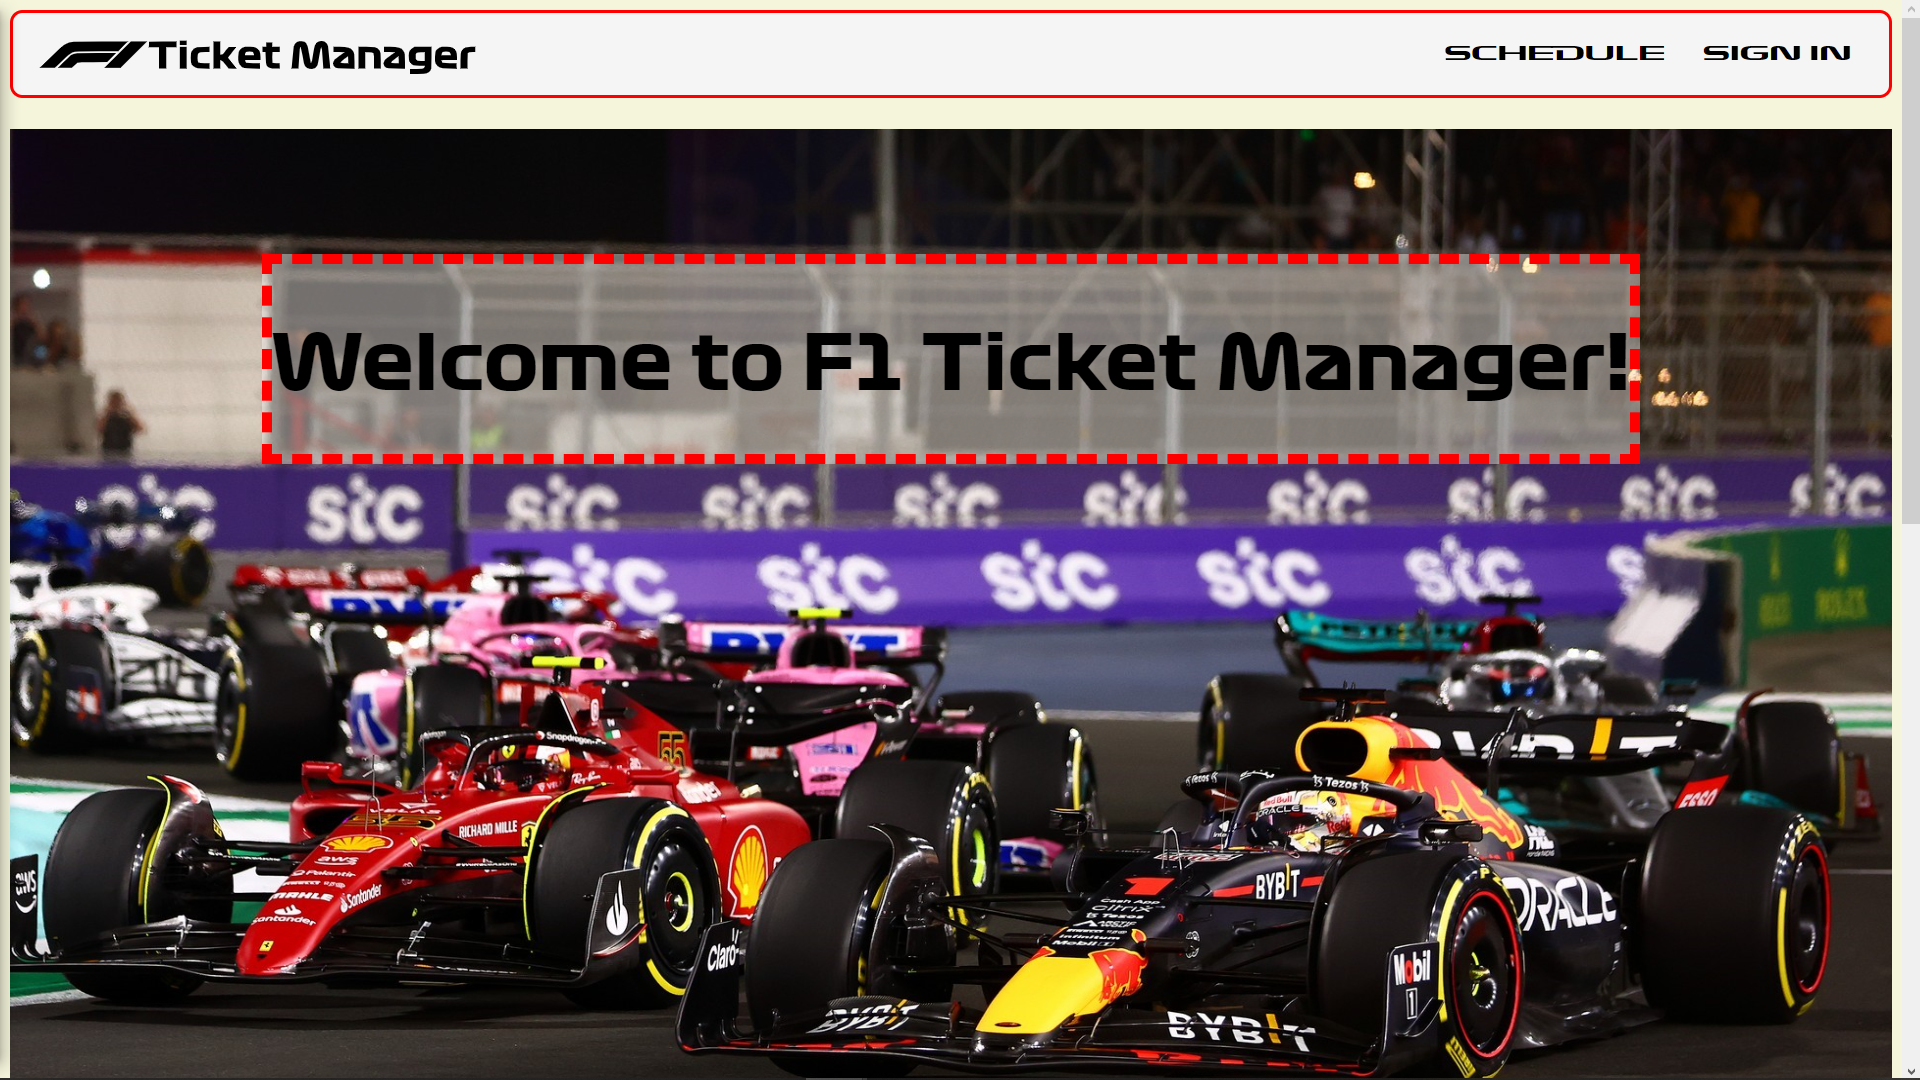
\includegraphics[scale=0.2]{images/homepage}
	\caption{Kezdőoldal}
	\label{abra:homepage}
\end{figure}
\pagebreak

\subsection {Versenynaptár (Schedule)}

A \textbf{Versenynaptár} oldalon lehet böngészni a 2022-es év versenyeinek listáját a megrendezési sorrendben. Az első kártya, ami megjelenik az oldalon az a következő verseny, amely automatikusan kerül ki az aktuális dátum alapján. Teszt jelleggel van egy dátum kiválasztó gomb is, hogy ki lehessen próbálni, hogy egy adott dátumhoz melyik verseny lesz a legközelebb. Erre a kártyára kattintva meg lehet tekinteni a részleteket. Minden kártyán látszanak a legfontosabb információk az adott versenyről, mint a pálya neve, a rendező ország neve, az intervallum, amikor az esemény zajlani fog és a pályarajz (\ref{abra:schedule}). Továbbfejlesztési lehetőség, hogy csak azok a pályák legyenek aktívak, amelyek még hátra vannak.

\begin{figure}[!h]
	\centering
	\begin{tabular}{cc}
	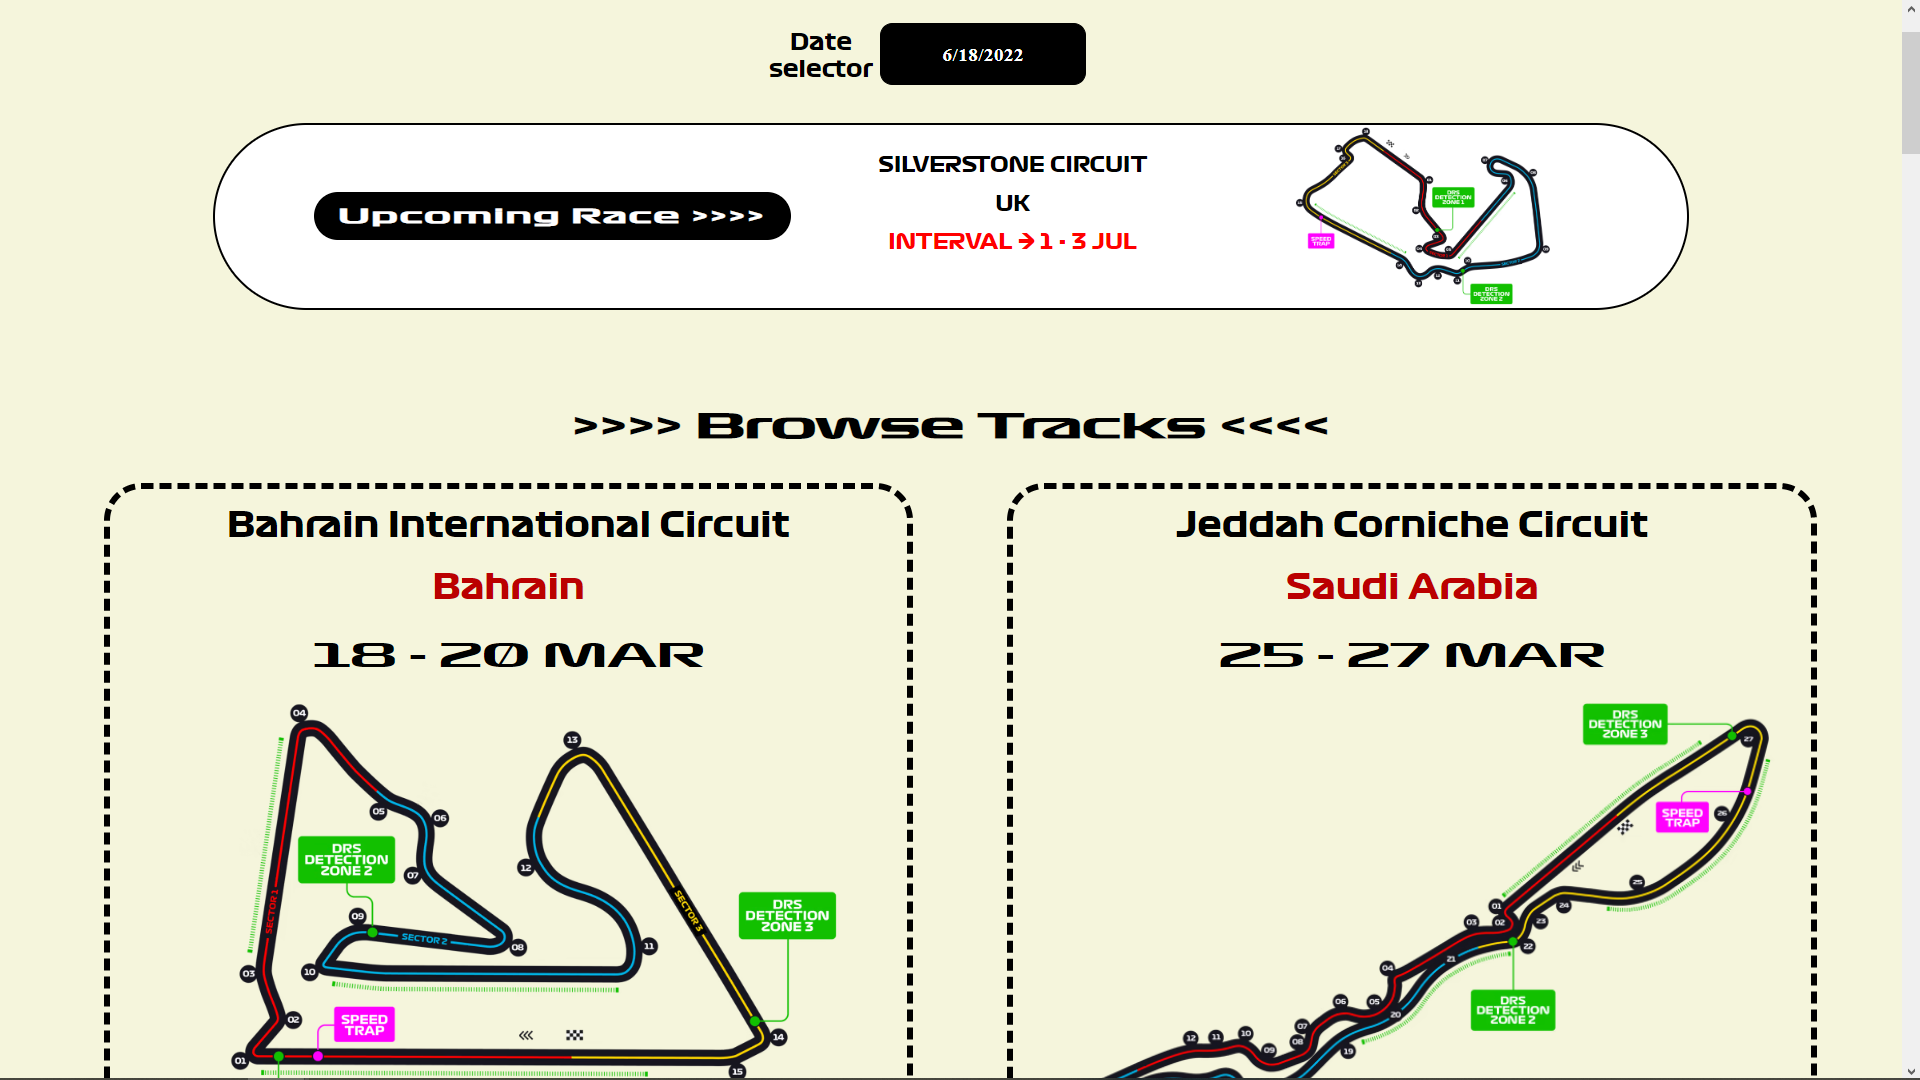
\includegraphics[scale=0.15]{images/schedule1} &
	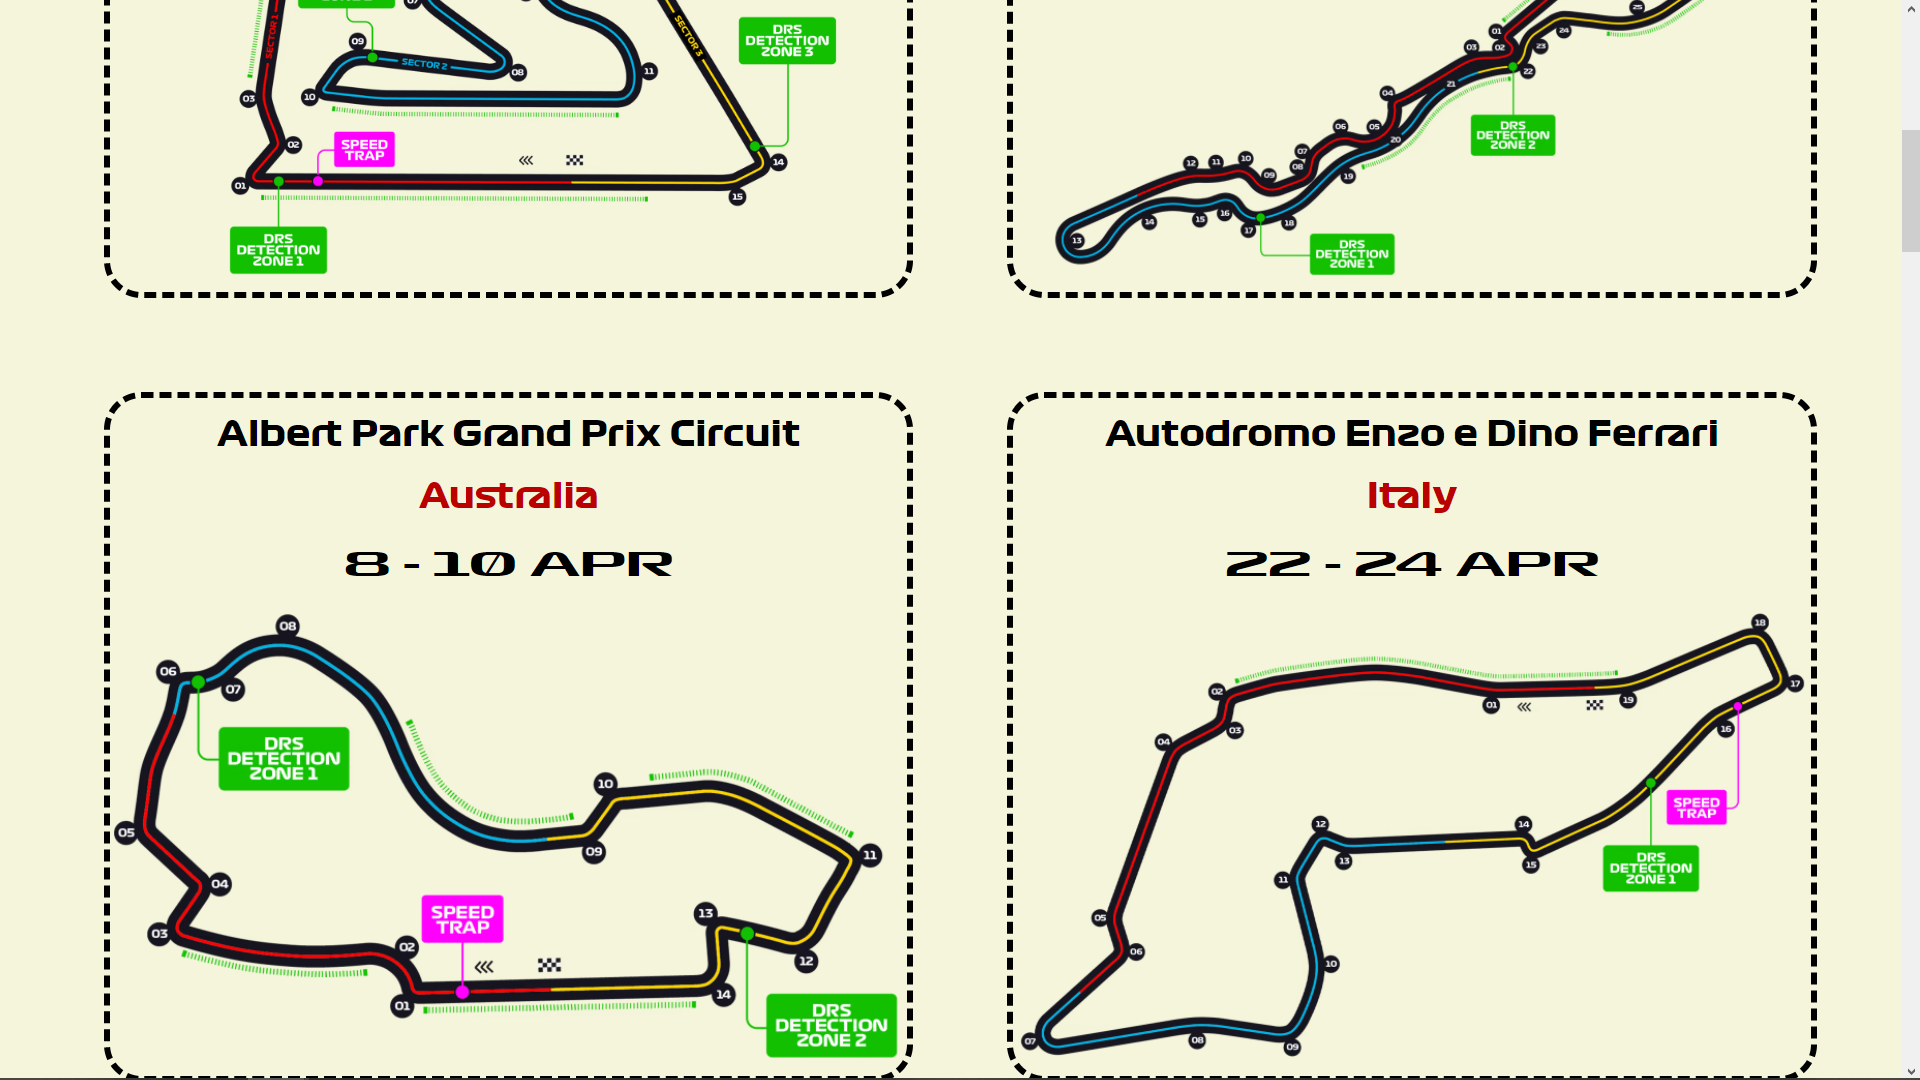
\includegraphics[scale=0.15]{images/schedule2} \\
	A versenynaptár & Görgetéssel látható az összes pálya
	\end{tabular}
	\caption{Versenynaptár}
	\label{abra:schedule}
\end{figure}

Ha átvisszük az egeret a kártya fölott, akkor megjelenik egy gomb \textbf{Browse tickets} szöveggel, amelyre kattintva megtekinthetőek a versenyhez tartozó jegy típusok és azok információi (\ref{abra:ticketsUA}). Ha nincs bejelentkezve a felhasználó, akkor az \textbf{Add to cart} gomb szürkén jelenik meg, vagyis nem lehet a kosárba tenni, viszont ha rákattint a felhasználó, akkor a rendszer jelezni fogja egy \textbf{alert} (figyelmeztetés) ablakban, hogy autentikáció szükséges, ha ezt a funkciót szeretné használni.

\begin{figure}[!h]
	\centering
	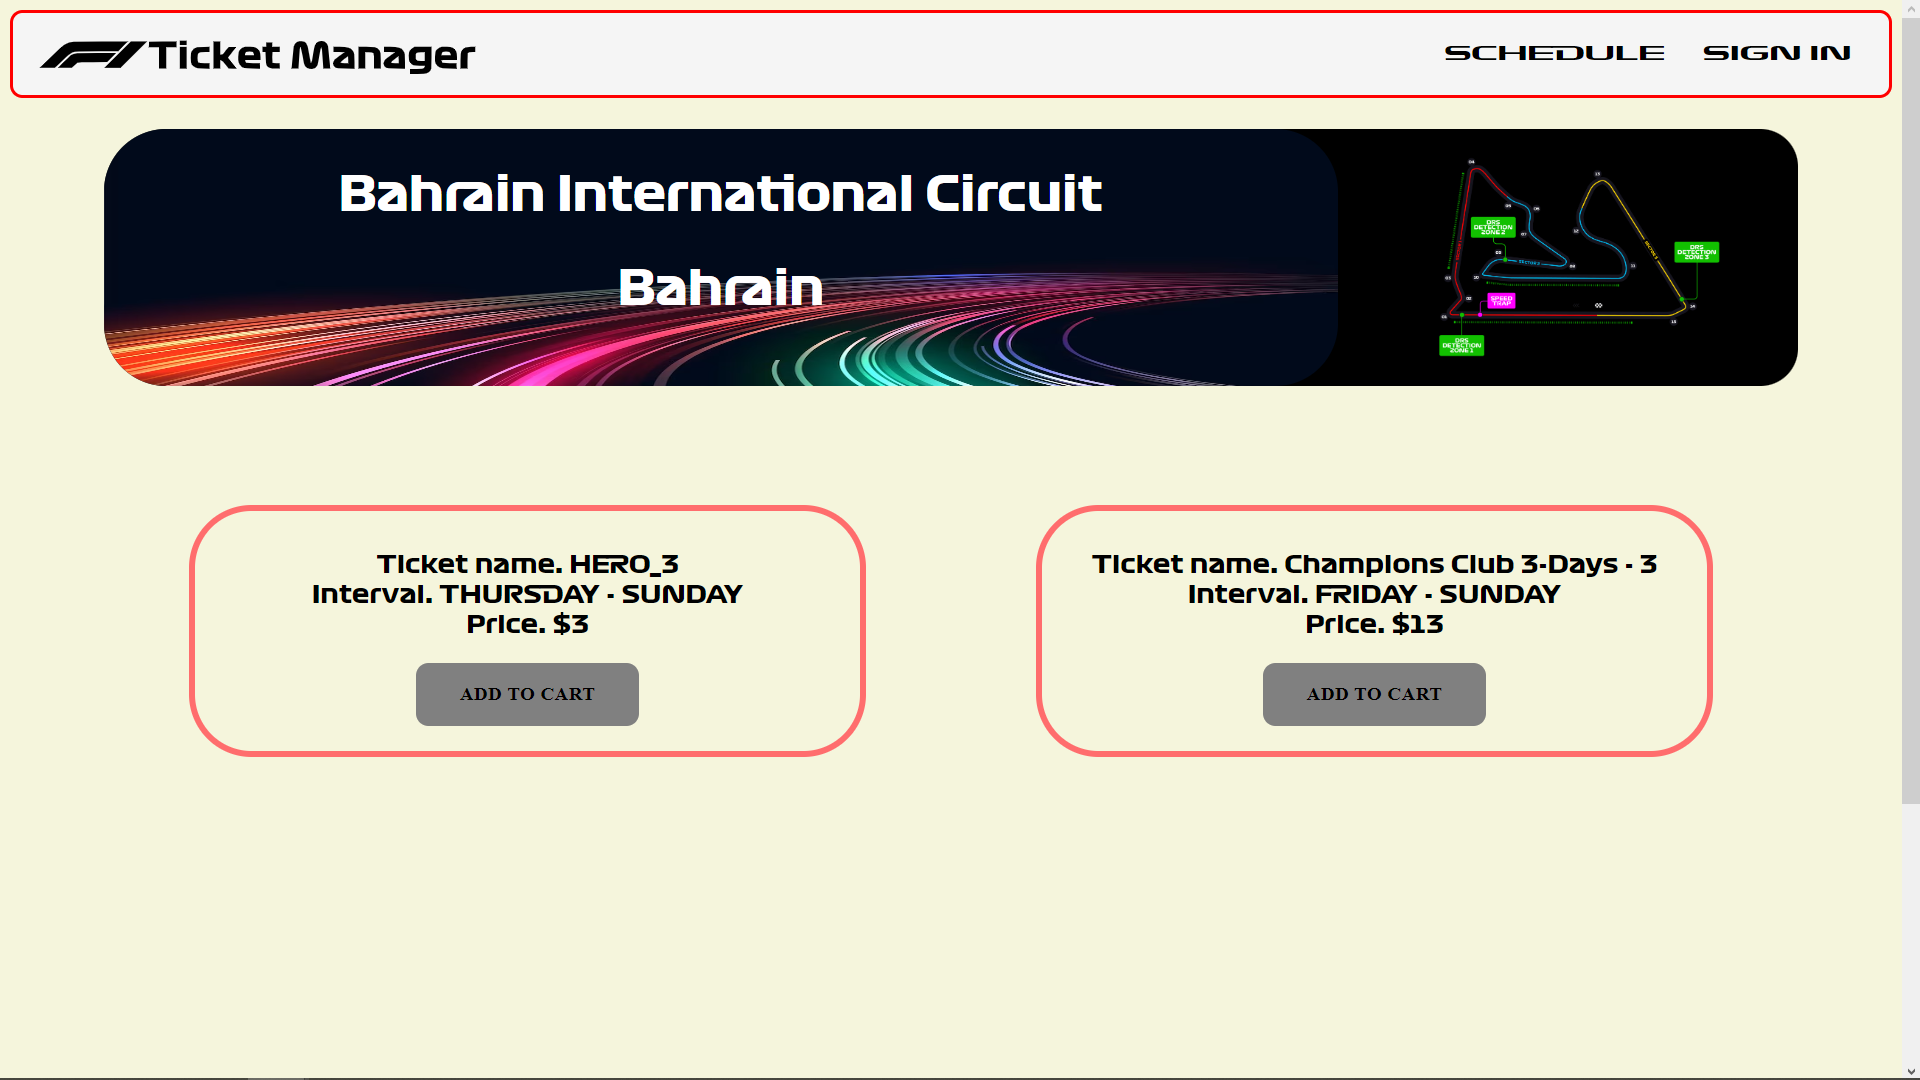
\includegraphics[scale=0.2]{images/tickets}
	\caption{Jegy típusok be nem jelentkezett felhasználóval}
	\label{abra:ticketsUA}
\end{figure}

Abban az esetben, ha a felhasználó be van jelentkezve, lehetőség van a jegyet a kosárba helyezni. Egy továbbfejlesztési lehetőség, hogy visszajelzést tudjon adni az adott jegyről, élményekről (\ref{abra:ticketsAuth}). A jegyek mennyiségét a \textbf{Checkout} oldalon van lehetősége módosítani a felhasználónak. A rendszer ezen része egy továbbfejlesztési terület, hogy adott esetben ellenőrizve legyen, hogy tényleg csak az tudjon visszajelzést adni, akkor vásárolt az adott jegyből. 

\begin{figure}[!h]
	\centering
	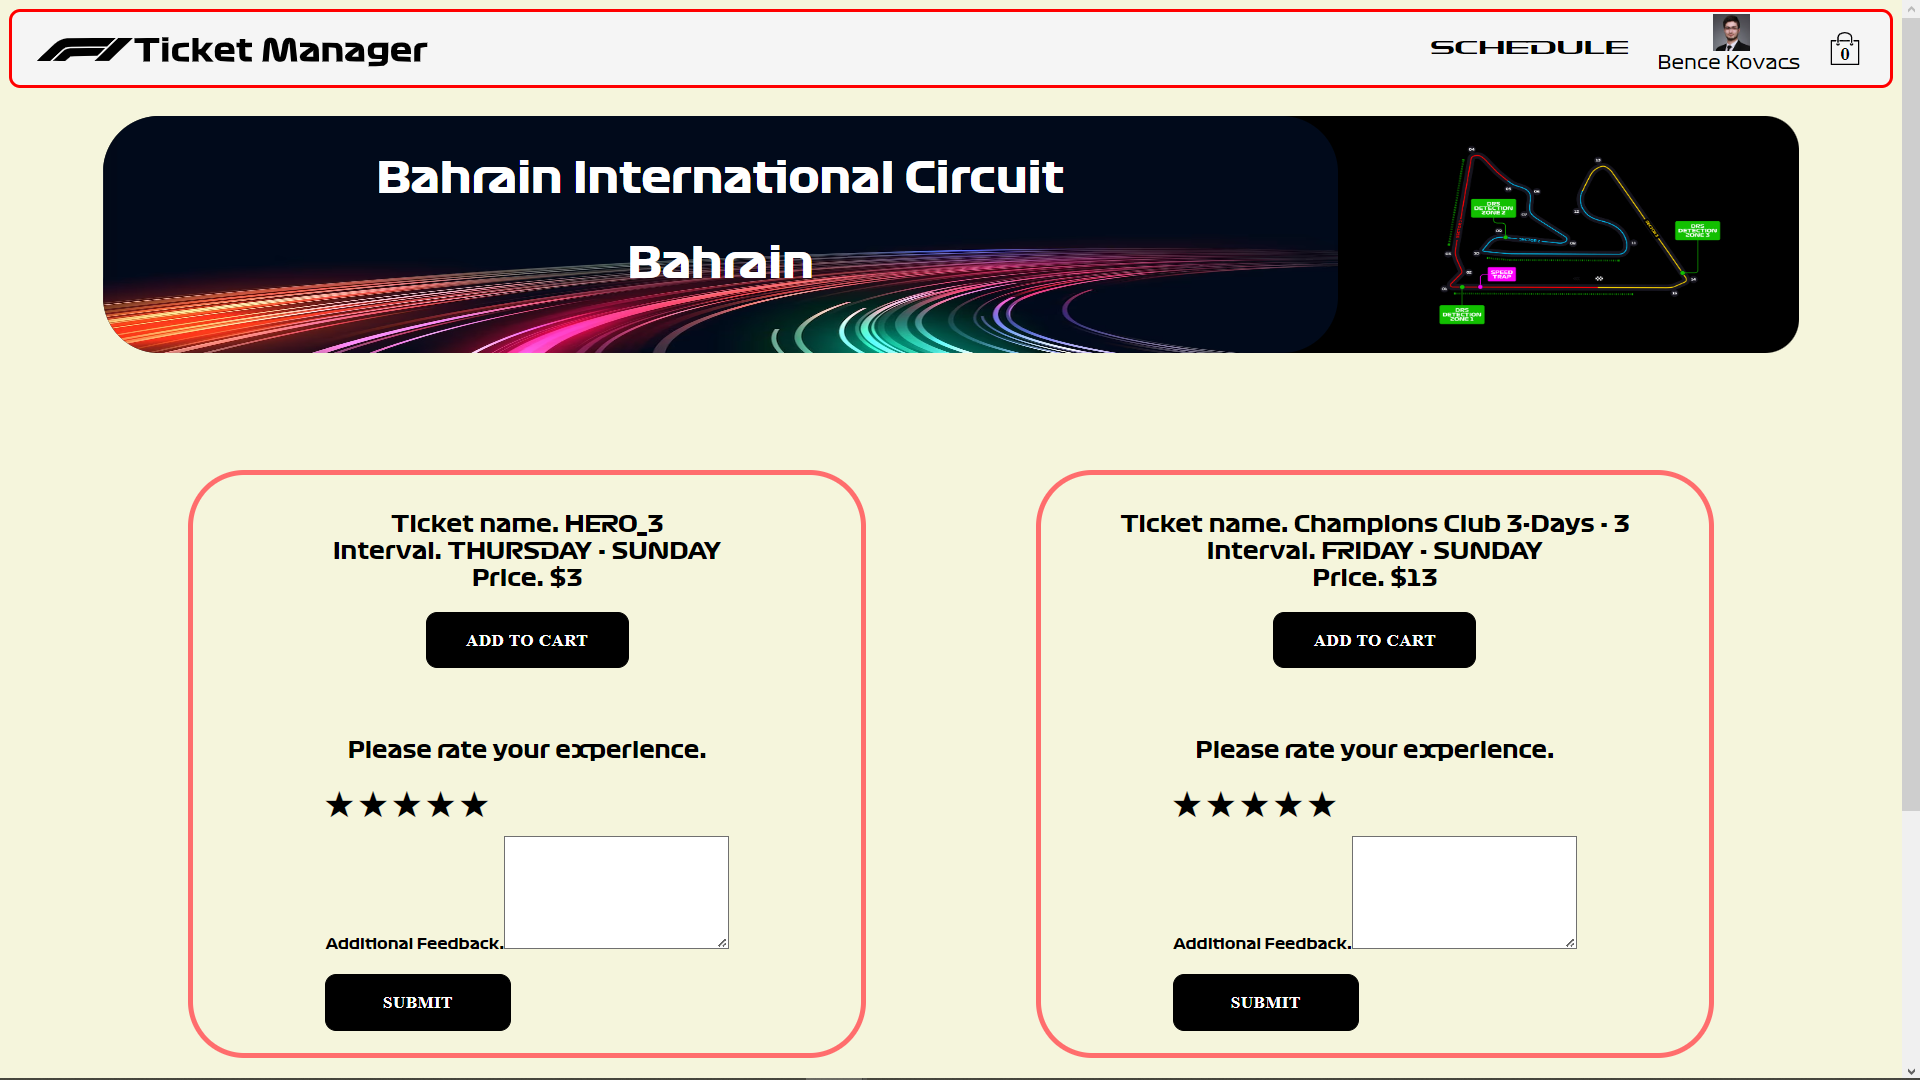
\includegraphics[scale=0.2]{images/ticketsAuth}
	\caption{Jegy típusok bejelentkezett felhasználóval}
	\label{abra:ticketsAuth}
\end{figure}

\subsection {Bejelentkezés és regisztráció (Sign in and up)}

A bejelentkezési felületen egyben lett feltüntetve a bejelentkezés és regisztráció két külön kártyán. Az email címmel vagy közösségi fiókkal való autentikáción kívül lehetőség van elfelejtett jelszó esetén új megadása. Ennek érdekében a felhasználó megadja az email címét és kapni fog egy levelet, amely tartalmaz egy linket az új jelszó megadásához (\ref{abra:signInUp}).

\begin{figure}[!h]
	\centering
	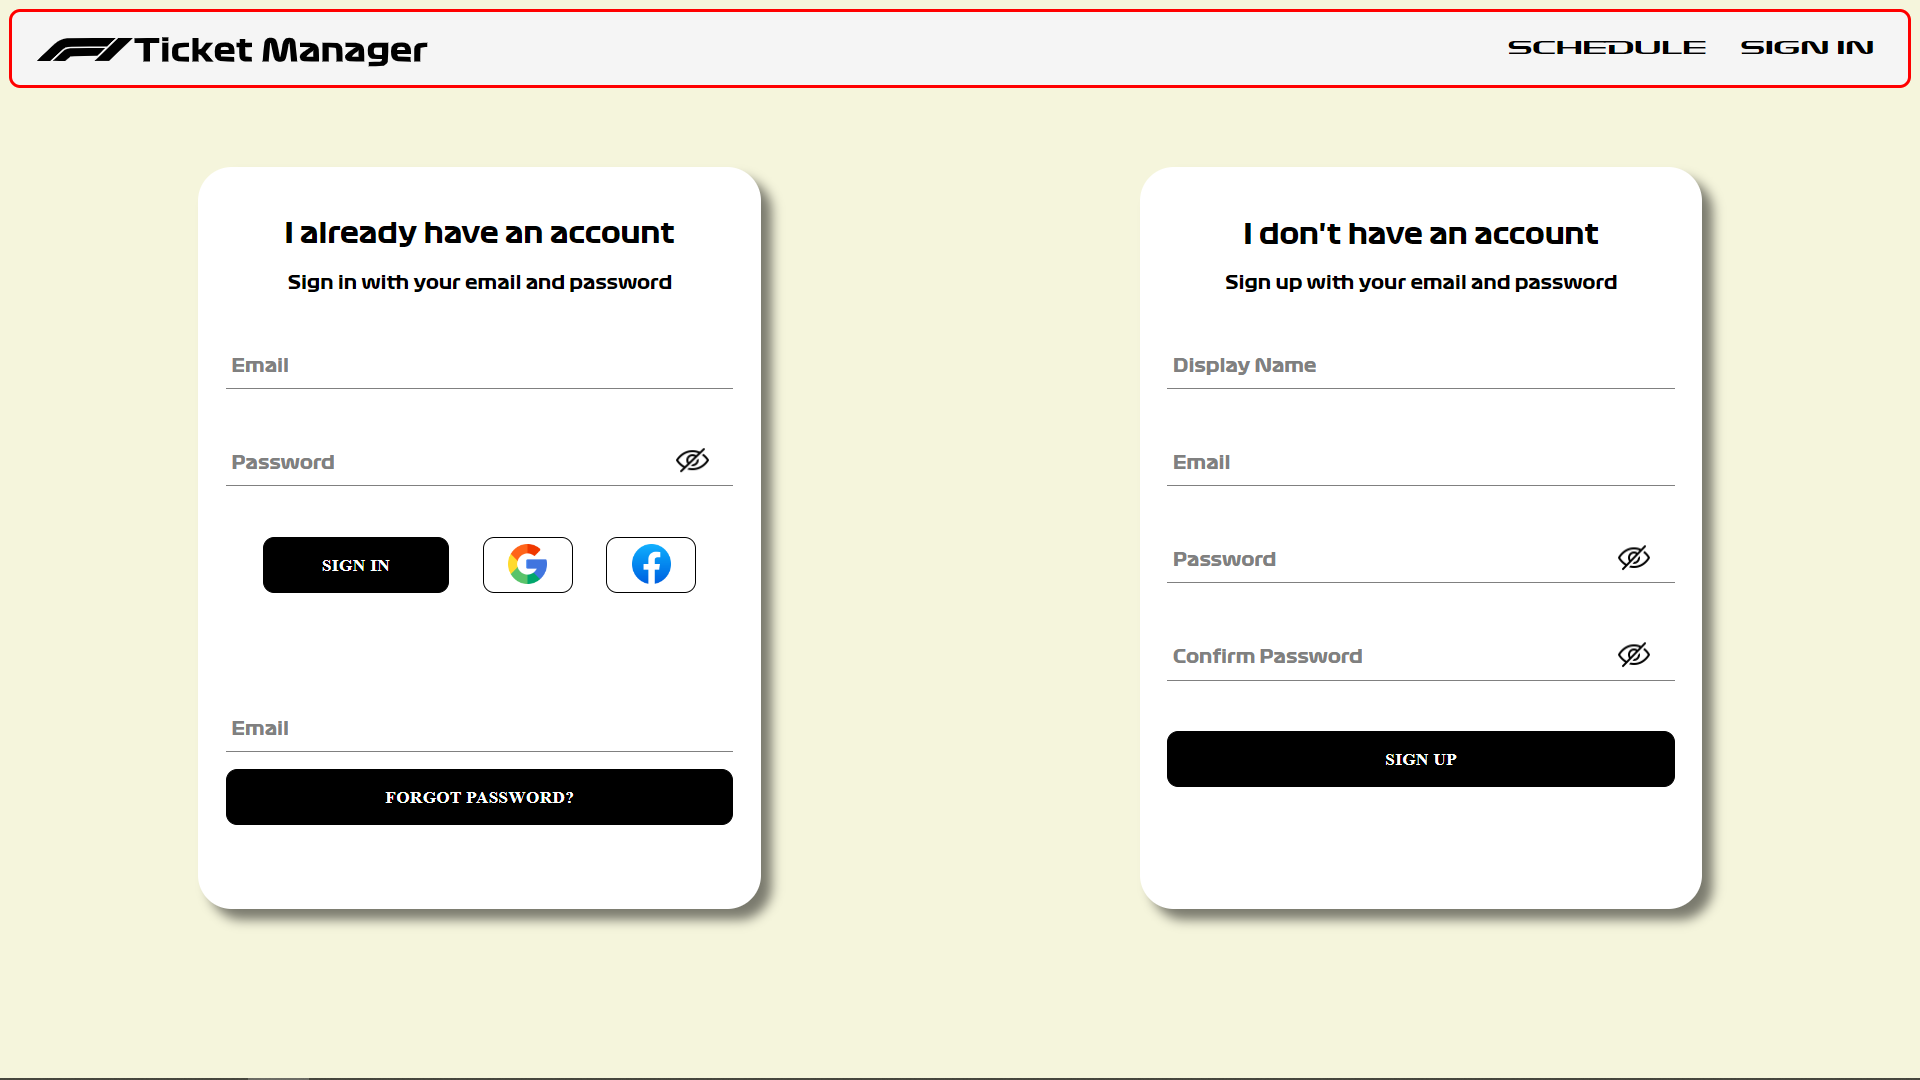
\includegraphics[scale=0.2]{images/signInUp}
	\caption{Autentikáció}
	\label{abra:signInUp}
\end{figure}

Továbbá lehetőség van a felületre való regisztrációra is a jobb oldali kártyán. Ennek a folyamatnak a bemutatására készítettem egy szekvencia diagramot a \textbf{SequenceDiagram.org} online szerkesztő segítségével \cite{Seq}.

\begin{figure}[!h]
	\centering
	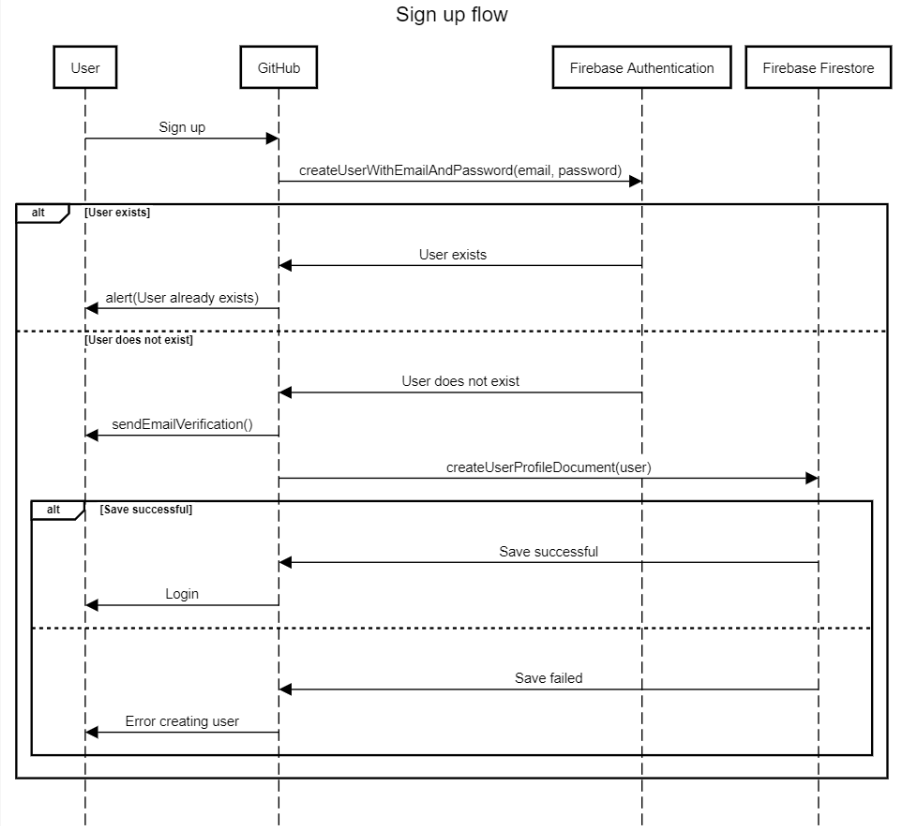
\includegraphics[scale=0.5]{images/signUpFlow}
	\caption{Szekvencia diagram - Regisztráció}
	\label{abra:signUpFlow}
\end{figure}
\pagebreak

A regisztráció folyamatát a felhasználó indítja el a kötelező mezők kitöltésével. A \textit{Firebase} szerver első sorban ellenőrzi, hogy az adott email címmel már létezik-e felhasználó és amennyiben igen, a megfelelő üzenetet jeleníti meg az oldal. Ellenkező esetben létrehozza a rendszerben a felhasználót, elmenti a megadott adatokat egyéb meta adatokkal kiegészítve, mint a létrehozás dátuma. A mentés után a rendszer automatikusan be is jelentkezteti a felhasználót (\ref{abra:signUpFlow}).

\subsection {Profil (Profile)}

A \textbf{Profil} oldal elérése csak a bejelentkezett felhasználóval lehetséges (\ref{abra:profile}). Ezen az oldalon lehetséges a profilkép és a megjelenített név módosítása az \textbf{Edit profile} gombra kattintva.

\begin{figure}[!h]
	\centering
	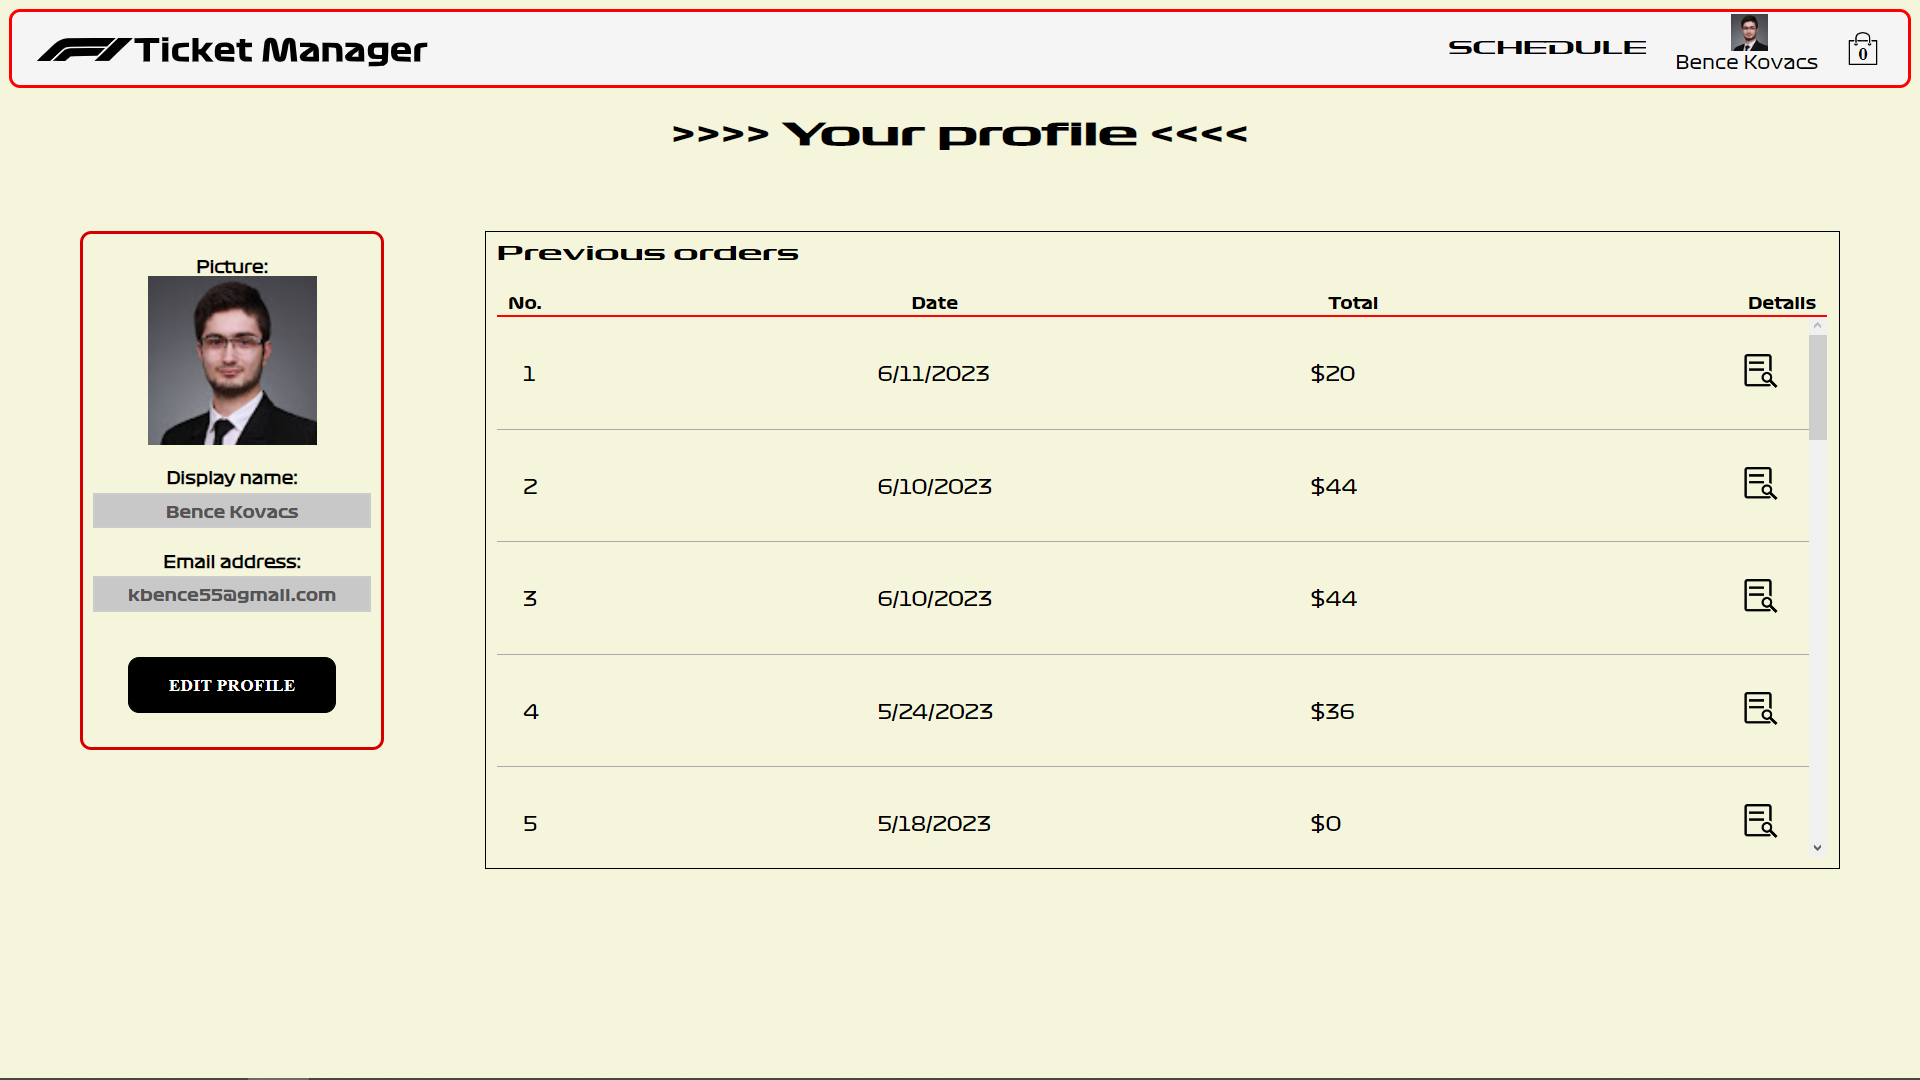
\includegraphics[scale=0.2]{images/profile}
	\caption{Saját profil oldal}
	\label{abra:profile}
\end{figure}

Az oldal jobb részén láthatóak a \textbf{rendelési előzmények}. Ezek görgetéssel böngészhetőek és a jobb szélén levő ikonra kattintva tekinthetőek meg a vásárlás részletei (\ref{abra:previousOrders}).

\begin{figure}[!h]
	\centering
	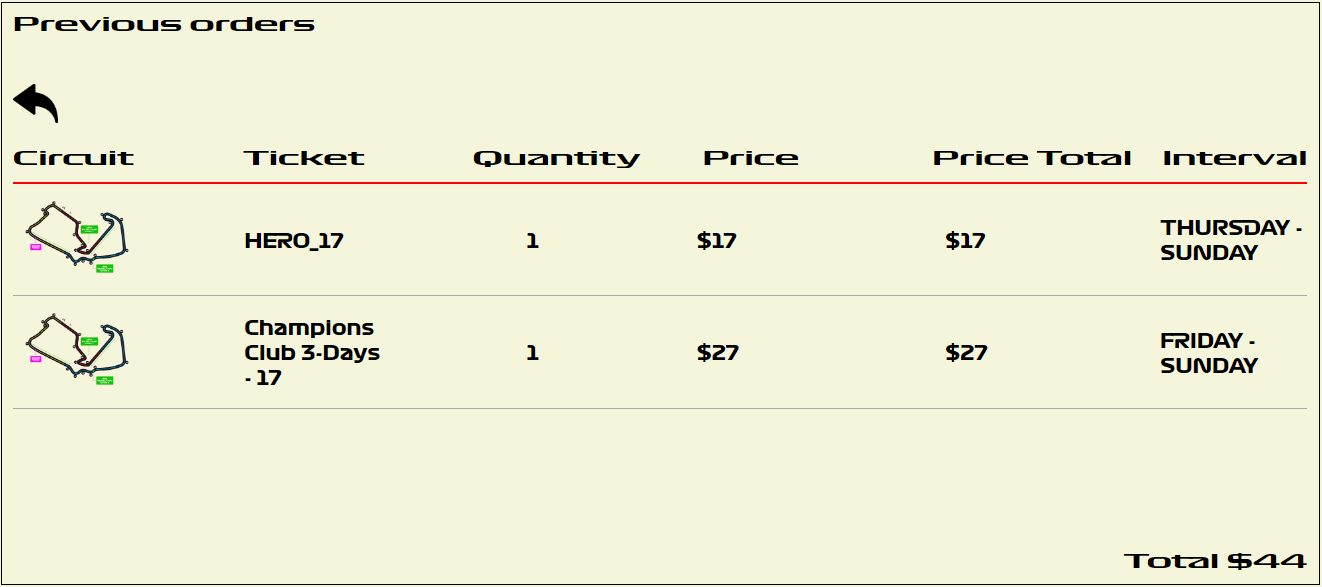
\includegraphics[scale=0.3]{images/previousOrders}
	\caption{Rendelés részletei}
	\label{abra:previousOrders}
\end{figure}

Amennyiben elvisszük valamely elem fölött az egeret megjelenik egy \textbf{More details} gomb, amelyre kattintva megtekinthető a jegy egyedi azonosítója (\ref{abra:moreDetails}). Ez a funkcionalitás azért fontos, mivel megtörténhet, hogy a felhasználó elveszíti vagy nem kapja meg a QR kódot emailben, ami ezt az azonosítót tartalmazza. Ha ez bekövetkezne, akkor innen is lehetőség van kimásolni és a megszokott módon azonosítani a PIN kóddal.

Ezen a felugró ablakon továbbá lehetősége van a felhasználónak egy új PIN kódot megadni, ha az aktuálist elfelejtette vagy úgy érzi, hogy valaki megszerezhette. Ezután egy újabb felugró ablakban lehetséges a PIN kód megváltoztatása. 

\begin{figure}[!h]
	\centering
	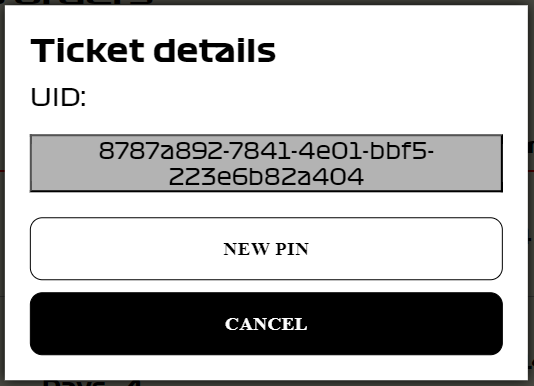
\includegraphics[scale=0.4]{images/moreDetails}
	\caption{Jegy részletei}
	\label{abra:moreDetails}
\end{figure}

A PIN kód megadásánál kötelezően egy 6 számjegyű számot kell megadni (\ref{abra:pinPopup}). Ezt manuálisan is be lehet írni vagy a \textit{pálca} ikonra kattintva generálódik egy véletlenszerű szám. A \textbf{Submit} gombra kattintva frissítheti a felhasználó a jegyhez tartozó kódot, ami teljes mértékben felülírja az előzőt, ezért nagyon figyelmes kell lenni a megadásakor, de erre a pirossal írt szöveg is figyelmezteti a vásárlót.

\begin{figure}[!h]
	\centering
	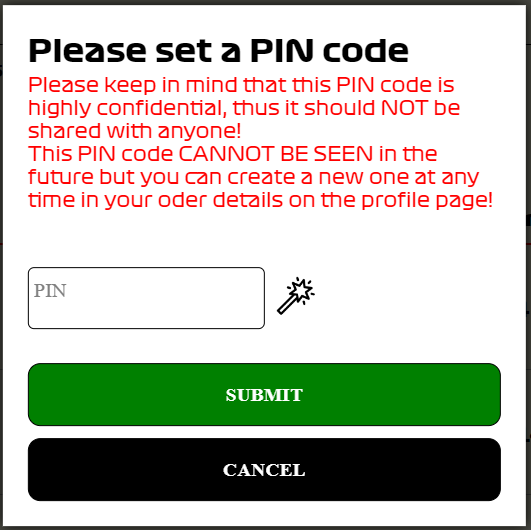
\includegraphics[scale=0.4]{images/pinPopup}
	\caption{PIN kód megadása}
	\label{abra:pinPopup}
\end{figure}
\pagebreak

\subsection {Rendelés (Checkout)}

A \textbf{Rendelés} oldalon van lehetősége a felhasználónak véglegesíteni a vásárlást (\ref{abra:checkout}). Itt is láthatóak a kosárba helyezett jegyek információi és csak itt módosíthatóak az egyes jegyek mennyisége vagy a kosárból való törlése. A \textbf{Pay Now} gombra kattintva a felhasználó meg tudja adni a számlázási adatokat majd a kártyaadatokat a vásárlás véglegesítéséhez. Ezt a \textbf{Stripe} szolgáltatás segítségével valósítottam meg. Sikeres vásárlás esetén a felhasználónak küld a rendszer egy emailt, amiben megkapja a QR kódokat. Egy kód tartalmazza a rendelés egyedi azonosítóját kombinálva a felhasználó egyedi azonosítójával. Az emailek küldésére a \textbf{Brevo} szolgáltatót vettem igénybe \cite{Brevo}.

\begin{figure}[!h]
	\centering
	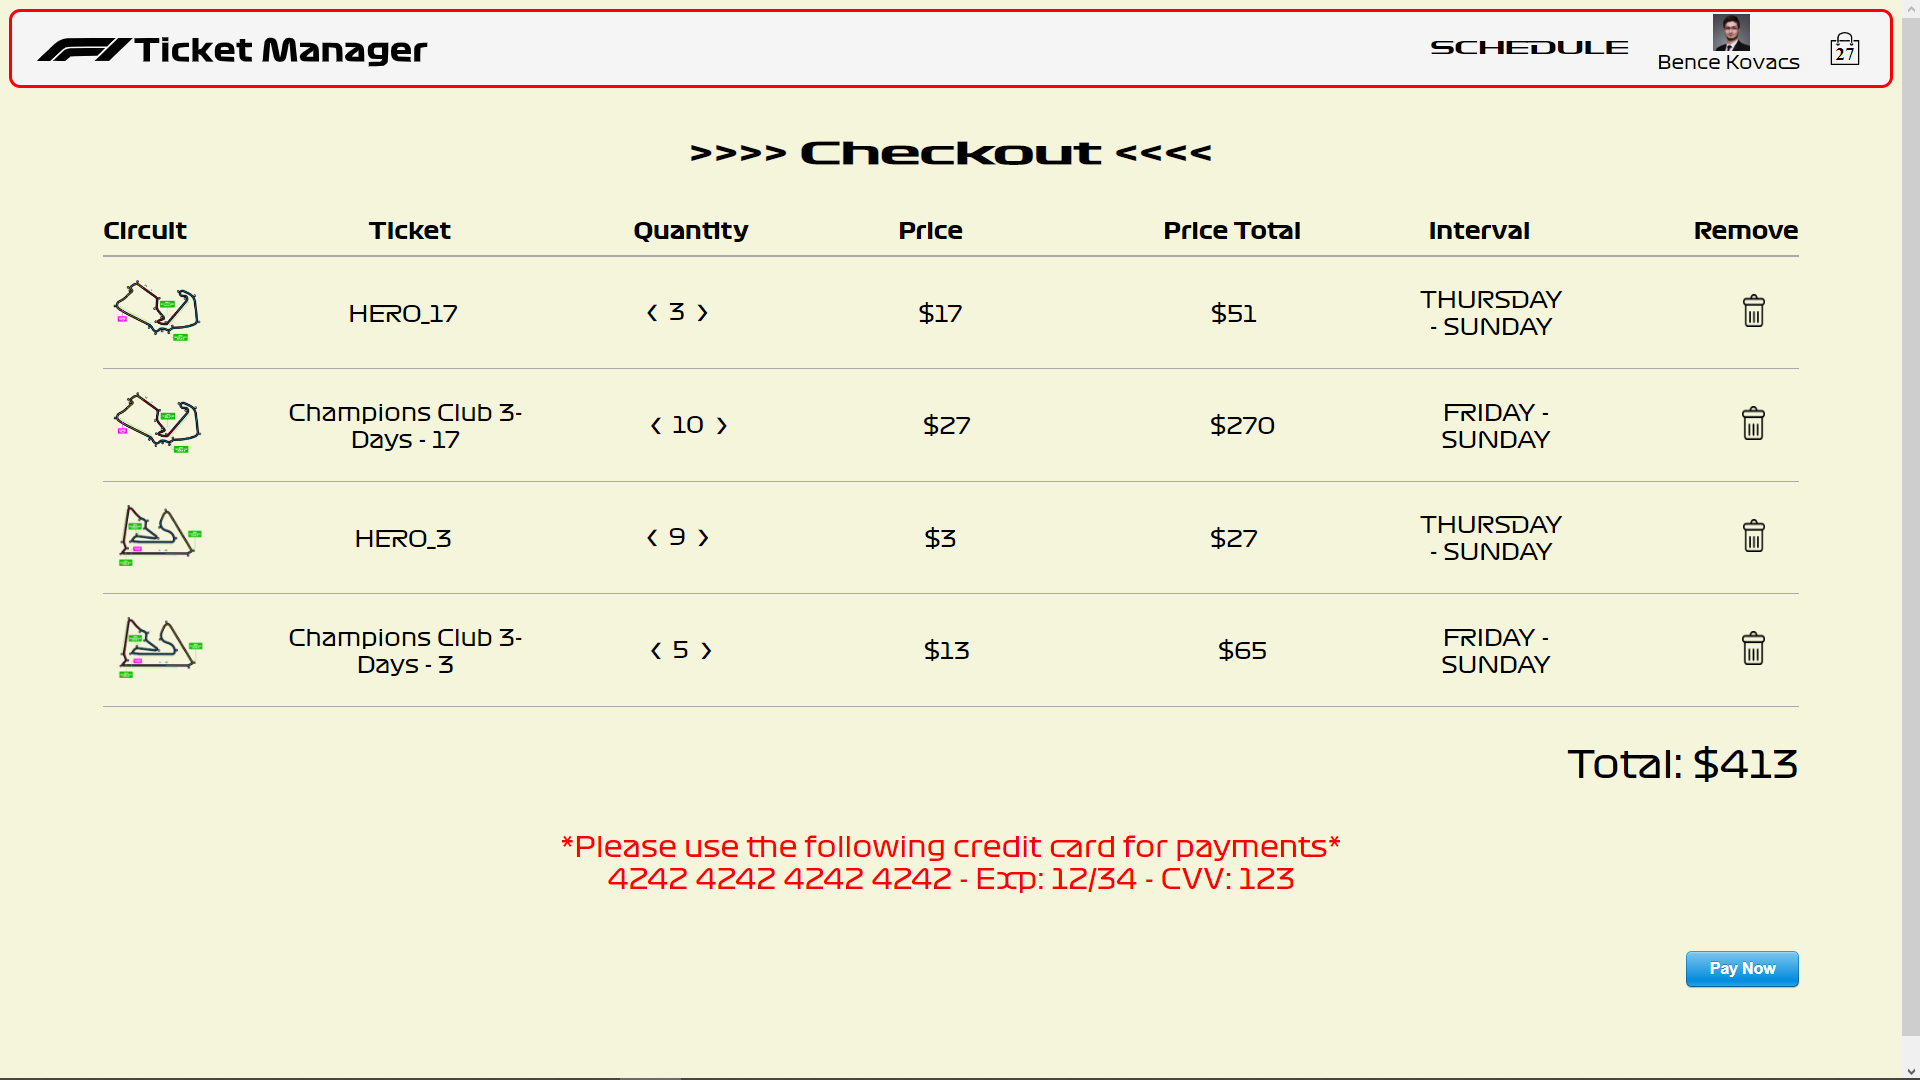
\includegraphics[scale=0.2]{images/checkout}
	\caption{Rendelés véglegesítése}
	\label{abra:checkout}
\end{figure}

A rendelés leadása után az adatok eltárolására használt titkosítás elvégzésére több megoldást is kipróbáltam, amelyek közül az egyik az \ref{code:encryption} kódrészlet, amely az AES algoritmus egyik használati módja JavaScript programozási nyelven a CryptoJS könyvtárcsomag segítségével.

A kód első lépése a \textit{salt (só)} generálása, ami egy 128/8 bájt szekvencia, amely segítségével meghatározásra kerül majd a key (kulcs). A \textit{CryptoJS.lib.WordArray.random(128 / 8)} kódsor a \textbf{CryptoJS} könyvtárban található \textit{random()} függvény hívásával egy véletlenszerű 128-bites szekvenciát generál, majd beilleszti az adatokat a WordArray osztályba.

A következő lépésben a kulcs előállítása történik meg a \textit{secretPass (jelszó)} és a só használatával a kulcsderiváló függvény segítségével. A kulcs előállítása a \textit{CryptoJS.PBKDF2()} függvénnyel történik, amely egy kulcstervező függvény. Az első paraméter a titkosításhoz használt jelszó, a második argumentum a só, a harmadik pedig a kulcs hosszát és az iterációk számát határozza meg. Ennél az algoritmusnál nagyon fontos odafigyelni, hogy a jelszó szigorúan titkos információ, vagyis ezt biztonságosan ajánlott eltárolni szerver oldalon. A többi paraméter publikus, mert önmagukban nem elegendőek a titkosított szöveg visszafejtéséhez.

Az inicializáló \textit{vektor (iv)} generálása következik. Az IV egy véletlenszerű bájt szekvencia, amelynek hossza megegyezik a blokk méretével (128 bit), és a titkosítás során használják, hogy azonos adatok esetén is véletlenszerű kimenetet generáljon.

Az adat titkosítása a \textit{CryptoJS.AES.encrypt()} függvénnyel történik. Az adatot először JSON formátumba alakítjuk, majd az AES algoritmust a kulcs, az IV és további paraméterek (mód, padding és tag) megadásával alkalmazzuk. A \textit{mode} a blokktitkosítási mód (BCM) kiválasztására szolgál, ezek között található a ECB, CBC, OFB vagy CFB. A mi esetünkben a CBC (Cipher Block Chaining) mód van használva.

\begin{lstlisting}[caption={Titkosítás példakód.}, captionpos=b, language = JavaScript, label={code:encryption}]
export const encryptData = text => {
  const salt = CryptoJS.lib.WordArray.random(128 / 8);
  const key = CryptoJS.PBKDF2(secretPass, salt, {
    keySize: 256 / 32,
    iterations: 1000,
  });
  const iv = CryptoJS.lib.WordArray.random(128 / 8);

  const encrypted = CryptoJS.AES.encrypt(JSON.stringify(text), key, {
    iv: iv,
    mode: CryptoJS.mode.CBC,
    padding: CryptoJS.pad.Pkcs7,
    tag: true,
  });

  const data = {
    ciphertext: encrypted.ciphertext.toString(CryptoJS.enc.Base64),
    iv: iv.toString(CryptoJS.enc.Base64),
    salt: salt.toString(CryptoJS.enc.Base64),
    tag: true,
  };
  return JSON.stringify(data);
};
\end{lstlisting}

A \textit{padding} a blokkok kitöltési módját határozza meg, itt a \textbf{Pkcs7} (Public Key Cryptography Standards 7-es szabványa) van használva. A Pkcs7 padding szabvány szerint, ha az üzenet hossza nem egész blokk méretű, akkor azt szükséges kiegészíteni. Minden hiányzó bájt felveszi a hiányzó bájtok számának megfelelő értéket. Ha például az utolsó blokkban 3 hiányzó bájt van, akkor a blokk utolsó bájtjai a 0x03 értéket veszi fel.

Az \textit{iv} az inicializáló vektort tartalmazza, amit korábban generáltunk. A \textit{tag} beállítása igazra van állítva, hogy az üzenet hitelesítése (integritásának ellenőrzése) is megtörténjen a titkosítás során. A tag az üzenet elejére kerül beillesztésre a titkosítás során, és végül az eredeti üzenet végén kerül ellenőrzésre a helyessége.

Az utolsó lépés a \textit{titkosított adat (ciphertext)}, az IV, a só és az üzenet hitelesítésének értéke (tag) összekapcsolása és JSON formátumba rendezése és visszatérítése.

Az alábbi példakód a visszafejtést valósítja meg (\ref{code:decryption}):

\begin{lstlisting}[caption={Visszafejtés példakód.}, captionpos=b, language = JavaScript, label={code:decryption}]
export const decryptData = text => {
const json = JSON.parse(text);
const salt = CryptoJS.enc.Base64.parse(json.salt);
const iv = CryptoJS.enc.Base64.parse(json.iv);
const tag = json.tag;
const ciphertext = CryptoJS.enc.Base64.parse(json.ciphertext);

const key = CryptoJS.PBKDF2(secretPass, salt, {
	keySize: 256 / 32,
    	iterations: 1000,
});

const decrypted = CryptoJS.AES.decrypt(
  	{ ciphertext: ciphertext, salt: salt, iv: iv, tag: tag },
    	key,
    	{
     	iv: iv,
      	mode: CryptoJS.mode.CBC,
      	padding: CryptoJS.pad.Pkcs7,
      	tag: true,
    }
  );
  return JSON.parse(decrypted.toString(CryptoJS.enc.Utf8));
};
\end{lstlisting}

A \textbf{decrypt} függvény az \textbf{encrypt} függvénnyel ellentétes sorrendben dolgozza fel az adatokat. A paraméterként kapott titkosított szövegből JSON objektumot állít elő. Ezután ebből az objektumból megkapja a só és az iv Base64 formátumból az értékeket. A kulcs előállítása a \textit{PBKDF2} függvénnyel történik a jelszó és a só segítségével. A titkosított adat, az iv, a só és a hitelesítési tag felhasználásával sikeresen vissza tudjuk fejteni az eredeti üzenetet.

A másik opció a \textbf{CryptoJS} csomag mellett a \textbf{node-rsa} könyvtárcsomag segítségével megvalósított titkosítás és RSA kulcscsere volt \textbf{NodeJS} keretrendszerben. A \ref{code:rsaEncrypt} kódrészletben az adat titkosítása látható a RSA publikus kulcs segítségével (\ref{code:rsaGenrerate} kódrészlet), amelyet minden rendelés során a rendszer generál a privát kulcs mellett. A titkosítás során szükség van a \textit{publicKey}-re, amely a generálás során elmentődik az adatbázisba és ezt lekéri a rendszer. A publicKey segítségével titkosítom az \textit{AES} kulcsot, amellyel titkosítom az eredeti szöveget. A végeredmény egy \textbf{encryptedData} és egy \textbf{encryptedKey} lesz, amelyek hasonlóan bekerülnek az adatbázisba az összesített rendelések közé, az \textbf{orders} dokumentumba.

\begin{lstlisting}[caption={RSA kulcscsere és titkosítás.}, captionpos=b, language = JavaScript, label={code:rsaEncrypt}]
const aesKey = CryptoJS.lib.WordArray.random(16).toString();
const encryptedData = CryptoJS.AES
	.encrypt(<unique code with PIN code>, aesKey).toString();

const rsaKey = new NodeRSA();
rsaKey.importKey(publicKey, "public");
const encryptedKey = rsaKey.encrypt(aesKey.toString(), "base64");
\end{lstlisting}

\begin{lstlisting}[caption={RSA kulcsok generálása.}, captionpos=b, language = JavaScript, label={code:rsaGenrerate}]
const key = new NodeRSA({ b: 2048 });
const publicKey = key.exportKey("public");
const privateKey = key.exportKey("private");
\end{lstlisting}

A \ref{code:rsaDecrypt} kódrészletben lekéri a rendszer a rendeléshez tartozó privát kulcsot, majd annak segítségével visszafejti a titkosított \textit{AES} kulcsot. Ezzel a kulccsal már vissza lehet fejteni a titkosított szöveget, ezáltal megkapni a az eredeti szöveget az egyedi azonosítóval és a PIN kóddal.

\begin{lstlisting}[caption={RSA visszafejtés.}, captionpos=b, language = JavaScript, label={code:rsaDecrypt}]
const rsaKey = new NodeRSA();
rsaKey.importKey(privateKey, "private");
const decryptedKey = rsaKey.decrypt(data?.encryptedKey, "utf8");

const decryptedData = CryptoJS.AES.decrypt(
	data?.encryptedData,
	decryptedKey
).toString(CryptoJS.enc.Utf8);
\end{lstlisting}

\pagebreak
\subsection {Beléptetés (Scan)}

A \textbf{Beléptetés} oldalon a rendszer \textit{Adminisztrátora(i)} tudják a jegyeket hitelesíteni a versenyhelyszíneken az erre a célra kihelyezett termináloknál (\ref{abra:scan}). A felhasználó a kamera elé helyezi a QR kódot \cite{RQR}, majd beírja a PIN kódot, amelyeket a rendszer rögzít és jelzi a hitelesítési folyamat eredményét.

\begin{figure}[!h]
	\centering
	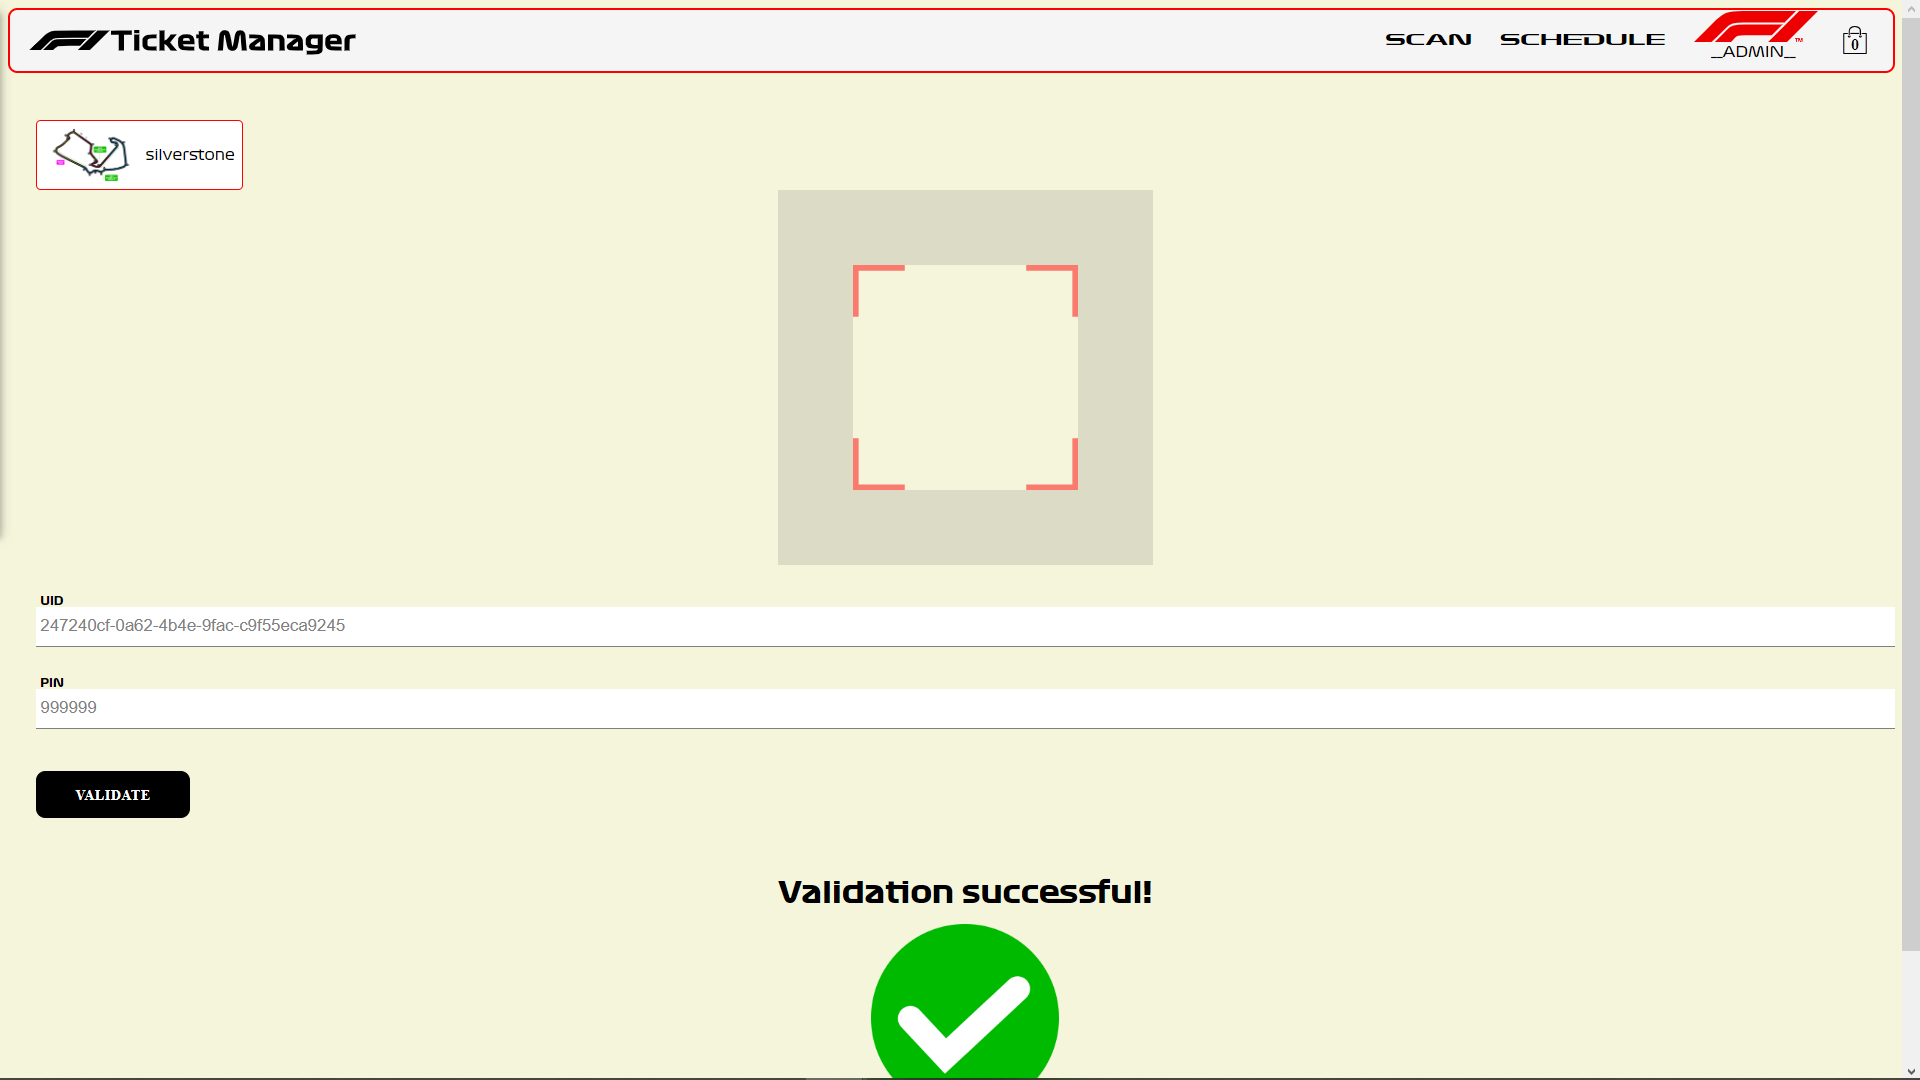
\includegraphics[scale=0.2]{images/scan}
	\caption{Jegyek hitelesítése}
	\label{abra:scan}
\end{figure}